\documentclass{emulateapj}
%\documentclass{aastex}
\submitted{{\it Submitted for publication in ApJL}}
\usepackage{multirow,color,wrapfig,ulem}
\usepackage {graphicx}

\usepackage{amsmath} 
\usepackage{amssymb} 
\usepackage{graphics}
\usepackage{epsfig}  
\usepackage{float}
\bibliographystyle{apj}
\def\be{\begin{equation}}
\def\ee{\end{equation}}
\def\ba{\begin{eqnarray}}
\def\ea{\end{eqnarray}}

\newcommand{\avg}[1]{\langle{#1}\rangle}  
\newcommand{\hMpc}{{\ifmmode{h^{-1}{\rm Mpc}}\else{$h^{-1}$Mpc }\fi}}  
\newcommand{\hGpc}{{\ifmmode{h^{-1}{\rm Gpc}}\else{$h^{-1}$Gpc }\fi}}  
\newcommand{\hmpc}{{\ifmmode{h^{-1}{\rm Mpc}}\else{$h^{-1}$Mpc }\fi}}  
\newcommand{\hkpc}{{\ifmmode{h^{-1}{\rm kpc}}\else{$h^{-1}$kpc }\fi}}  
\newcommand{\hMsun}{{\ifmmode{h^{-1}{\rm {M_{\odot}}}}\else{$h^{-1}{\rm{M_{\odot}}}$}\fi}}  
\newcommand{\hmsun}{{\ifmmode{h^{-1}{\rm {M_{\odot}}}}\else{$h^{-1}{\rm{M_{\odot}}}$}\fi}}  
\newcommand{\Msun}{{\ifmmode{{\rm {M_{\odot}}}}\else{${\rm{M_{\odot}}}$}\fi}}  
\newcommand{\msun}{{\ifmmode{{\rm {M_{\odot}}}}\else{${\rm{M_{\odot}}}$}\fi}}  
\newcommand{\kms}{{\ifmmode{{\mathrm{\,km\ s}^{-1}}}\else{\,km~s$^{-1}$}\fi}}
\newcommand{\bullb}{MACS J0025.4-1222}
\newcommand{\bulla}{1E0657---56} 
\shorttitle{Bullet Groups}
\shortauthors{Fern\'andez-Trincado et al.}

\begin{document} 

\title{Bullet Groups as a test of $\Lambda$CDM}
\author{J. G. Fern\'andez-Trincado$^{1,2,3}$, J. E. Forero-Romero$^1$
  and T. Verdugo$^3$} 
\affil{$^1$ Departamento de F\'{i}sica, Universidad de los Andes,
  Cra. 1 No. 18A-10, Edificio Ip, Bogot\'a, Colombia\\ 
       $^2$ Institute Utinam, CNRS UMR6213, Universit\'e de
  Franche-Comt\'e, OSU THETA de Franche-Comt\'e-Bourgogne,
  Besan\c{c}on, France\\ 
       $^3$ Centro de Investigaciones de Astronom\'ia, AP 264,
  M\'erida 5101-A, Venezuela}        

\begin{abstract}

We estimate the expected distribution of displacements between the two
dominant dark matter peaks in halos within a mass range corresponding
to galaxy groups. We find that the probability of finding a system
similar with displacements of $\sim$400 kpch$^{-1}$ is between 40\%
for z$=0$ and 60\% for z$=1$ and $\Lambda$CDM standard model, which
correspond to the observational constraint the object SL2S J08544-0121
that is  a gravitational lens found in the SL2S and located at
z$=0.35$. Given the larger abundance of groups with respect to
clusters, finding multi-modal groups and baryonic-dark matter
displacements.  
\end{abstract}

\begin{keywords}
{cosmology: theory -- dark matter} 
\end{keywords}

\section{Introduction}


The Bullet Cluster provided a new kind of observational evidence of
the existece of dark matter. Quantifying the displacement between dark
matter and the dominant baryonic component (hot X-ray emitting gas)
has been used to test the CDM paradigm itself by quantifying the
substructure velocity requiered to produce such displacement and also
by estimating the expected abundance of such events in the Universe.

Since that time there are other observations of other Bullet-like
systems [...].

Recently \citep{Gastaldello} observed baryonic-DM displacement if
$124\pm 20$ kpc in a group-like system with a total mass $2.4\pm 0.6
\times 10^{14}$\Msun. Systems of this mass are $\sim 10$ times more massive
than cluster systems in the mass range $>10^{15}$\hMsun, this opens
up the possibility of observationally finding bullet groups in a fair
amount to impose constraints on $\Lambda$CDM. This greater abundance
has to be weighted by the fraction of systems that present large
displacements. Such study has been performed for clusters but not for
lower mass systems.

In this Letter we present prediction for the abundance of group-like
systems that might show a DM-baryon displacement. To this end we use a
N-body cosmological simulation with such a resolution that allows us
to identify multimodal dark matter clumps in the circular velocity
range $300-1000$\kms. 

This paper is organized as the follows. In Section
\ref{sec:simulation} we present the simulation and the halo catalogs
used in this work. We continue in Section \ref{sec:setup} with the
geometry of the problem at hand and the measurements setup. Next in
Section \ref{sec:results} we present our results to finish with a
discussion and conclusion in Sections \ref{sec:discussion} and
\ref{sec:conclusions}. 


\section{Simulation and halo catalogs}
\label{sec:simulation}

We use the Bolshoi Run, a cosmological DM only simulation over a cubic
volume of 250 comoving \hMpc on a side. The simulation uses the ART code to
follow the evolution of  a dark matter density field sampled with
$2024^3$ from $z=80$ to $z=0$ [...]. The cosmology used  corresponds
to  the spatially flat concordance model with the following
parameters:  the density parameter for matter (dark matter$+$baryons)
$\Omega_m=0.27$, the density parameter for baryonic matter
$\Omega_b=0.0469$, the density parameter for dark energy
$\Omega_{\Lambda}=0.73$, the Hubble parameter $h=0.7$, the
normalization of the Power spectrum $n=0.95$ and the amplitude of mass
density fluctuation (at redshift z$=$0) $\sigma_8=0.82$.  The number
of particles used for each of the DM component was $2048^3$, resulting
in a mass resolution of $1.35 \times 10^8$
M$_{\odot}$h$^{-1}$. \citet{2011ApJ...740..102K}.  

\section{Bullet Geometry and Measurement Setup}
\label{sec:setup}

The configuration of the BGs in the simulations is shown in Figure
\ref{configuration}. There we depict a host and its most massive
sub-halo from in a particular case found at z$=0$. The arrows show the
position and the velocity vectors sub-halo in a frame of reference
where the main halo is at rest; thus  $\vec{v{}}=\vec{v}_{sub}-\vec{v}_{halo}$ and
$\vec{r}=\vec{r}_{sub}-\vec{r}_{halo}$.  The angle between these two
vectors characterized by,
\begin{equation}
  \mu\equiv \cos(\theta)=\frac{\vec{v{}}\cdotp{}\vec{r}}{\left\|v{}\right\| \left\|r\right\|}
 \end{equation} 
%
encodes the geometry of the collision, i.e. cases of $|\mu|\approx 1$
can be considered as head-on collisions while $|\mu|\approx 0$
describe a grazing trajectory.

The bullet-like encounter can be instantaneously described by
quantities the following quantities the circular velocity of the host
and the sub-halo, $V_{\rm c,host}$ and $V_{\rm c,  sub}$; the size of
the host halo $R_{\rm vir}$; the relative position and velocity of the
substructre, $\vec{v}$ and $\vec{r}$; and the angle between the
position and velocity $\mu$. 

Using these quantities one can describe three main stages in a
Bullet-like collision. First, the sub-halo crosses the virial radius
of the host halo in a head-on fashion, $|\vec{r}|/R_{\rm vir}\approx
1$ and $\mu\approx<0.0$. Second, as the sub-halo crosses for the first
time the center of the host halo $|\vec{r}|/R_{\rm vir} <
1.0$ and $\mu>0.0$. Third, as the sub-halo reaches apogee and
comes back to the center of the halo $|\vec{r}|/R_{\rm vir} < 1.0$ and
$\mu<0.0$.


the 
mass ranges and number of host halos and substructures 
are summary in the Table \ref{table1}. Of all the possible configurations that can be presented
in Figure \ref{configuration}, we are interested in estimate in the simulation the number 
of Bullet Groups that may be present in an Universe of 250 $h^{-1}$Mpc. For this we selected 
of the simulations all the substructures  
whose velocities indicate a movement out of the host halo. Each halo in this sample has a quantity
called $X_{off}$ that corresponds to the distance halo center (the minimum of the gravitational potential) to 
the center of mass normalized by the
virial radius ($R_{vir}$). Values of $X_{off}$
equal to zero indicate relaxed halos, while $X_{off}>0$ indicates the existence
of perturbed halos which can be considered candidates to be Bullet Groups and this ditribution is shown 
in a scatter plot in the Figure \ref{cos_theta1} and the distribution of $\nu_{circ,Halo}/\nu_{circ,Sub}$ 
is shown in  Figure \ref{cos_theta2}, both figures for differents z. 


\begin{table*}
\begin{center}
\begin{tabular}{ccccccc}\hline\hline
Sample       & Minimum $V_{\rm c}$         & Maximum $V_{\rm c}$          & \# Halos  & \# Halos  & \# Halos & \# Halos \\
             & \kms    & \kms  &   $z=0$   & $z=0.25$  & $z=0.5$  & $z=1$  \\\hline
Host   & 300\kms & XX &    400    &   362     &   310    &  192   \\ 
Sub-structure & 75\kms  & XX &    XX   &   XX     &   XX    &  XX   \\\hline
\end{tabular} 
\caption{Circular velocity ranges for the halos and subhalos at
  different redshifts.}  
\label{table1}
\end{center}
\end{table*}

\begin{figure}
\begin{center}
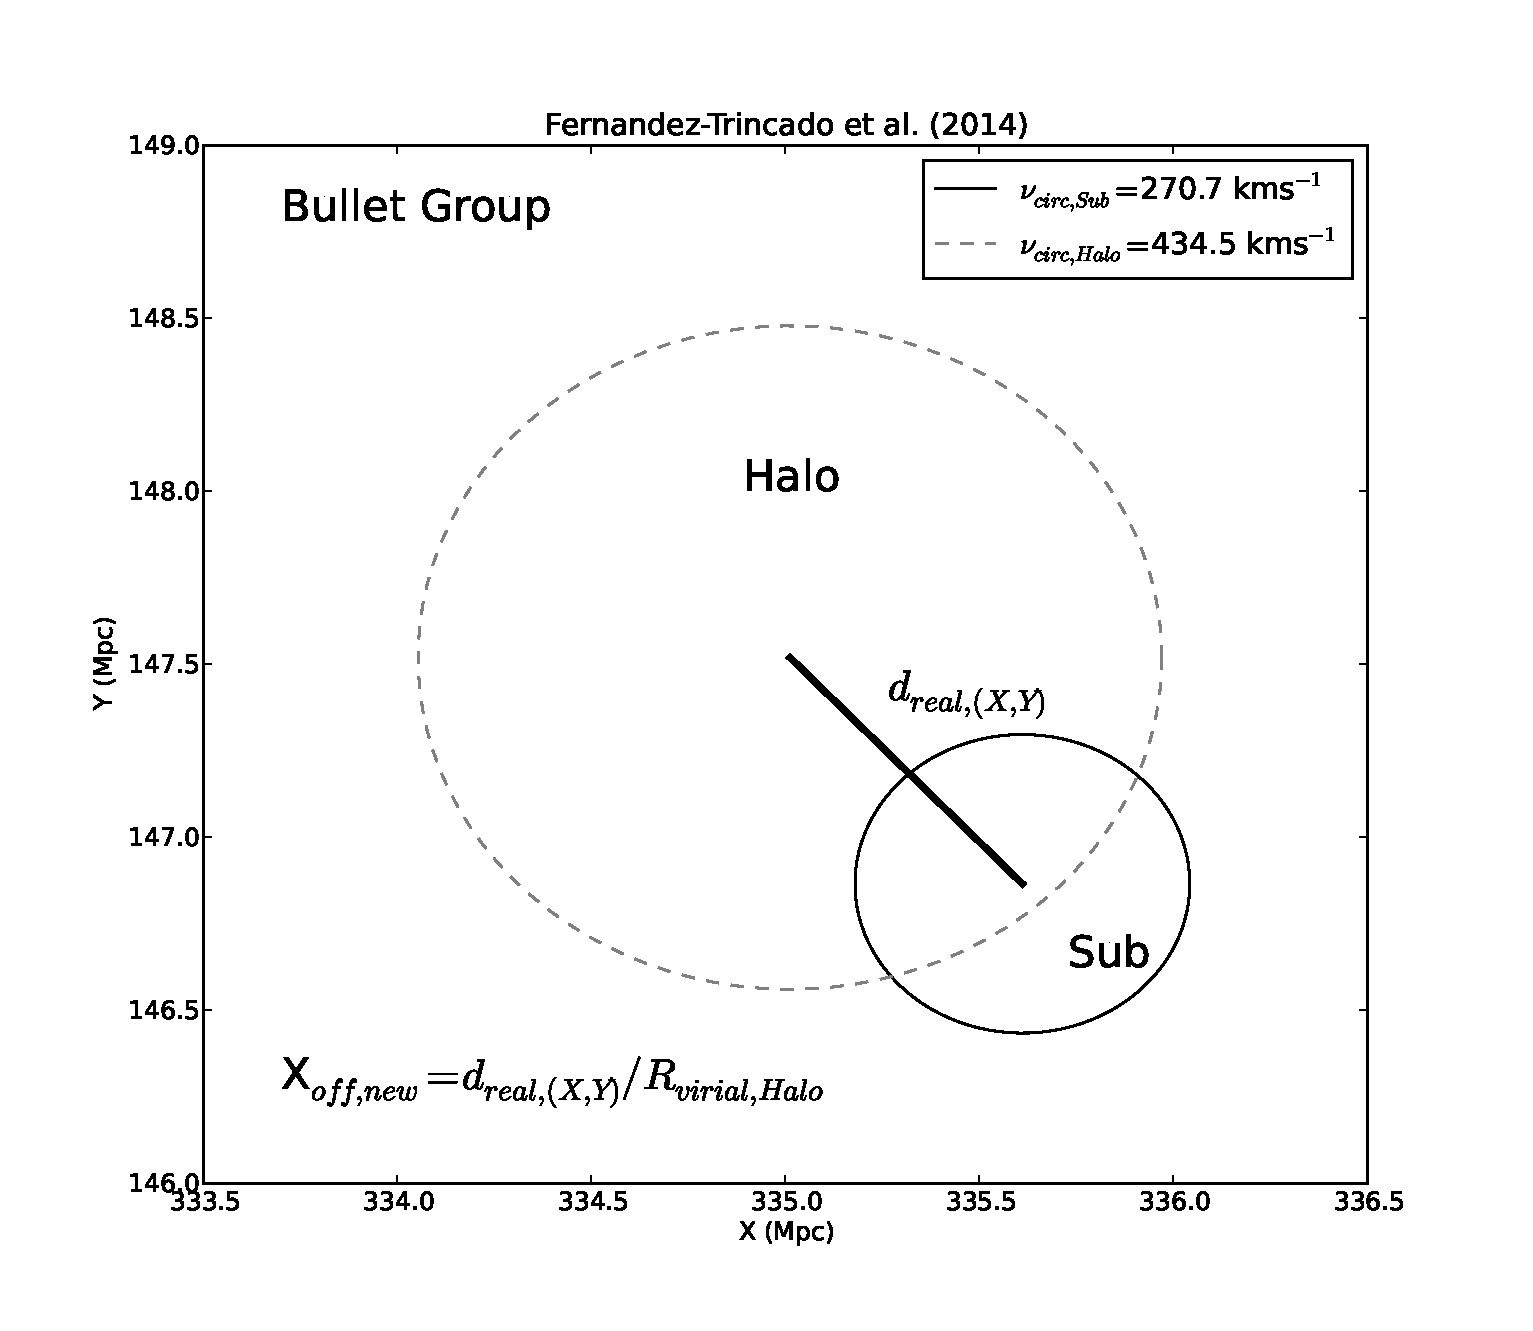
\includegraphics[width=0.45\textwidth]{Figures_eps/Bullet_Group.eps}
\end{center}
\caption{Configuration for a host halo (dashed circle) and
  sub-structure (black circle) in the sample.}  
\label{configuration}
\end{figure}




\begin{figure*}
\begin{center}
\includegraphics[width=1.0\textwidth]{Figures_eps/figure_5_4.eps}
\end{center}
\caption{Scatter plot for $X_{off}$ as function of the relation between velocities of substructures and the host halos and 
for different z. The top panel is represented to the sample with $v > 700$ \kms and down panel is represented 
for $v<700$ \kms} 
\label{cos_theta1}
\end{figure*}

\begin{figure*}
\begin{center}
%\includegraphics[width=1.0\textwidth]{Figures_eps/figure_5_2.eps}
\end{center}
\caption{Integrated distributions of $|\vec{v}|/V_{\rm c,host}$ at all
  $z$. The left panel correponds to the sample with $V_{\rm c, host}>700$ \kms and
  right panel correpond to the sample with $V_{\rm c,host}<700\kms$.} 
\label{cos_theta2}
\end{figure*}


\section{Results}
\label{sec:results}

\subsection{Cumulative Probability Distributions}
\label{cumulative_distribution}

We selected four snapshot of the simulation for four different
redshifts (z$=0$, z$=0.25$, z$=0.5$ and z$=1$) based in the
distribution of redshift in the Figure 1 by \citet{verdugo}, and  for
each sample in redshift we selected the host halo with circular
velocities greater than 300 kms$^{-1}$ and was split in two  principal
groups: The first group correspond to host halo with circular
velocities between 300 kms$^{-1}$ to 700 kms${^{-1}}$ with mass in the
range of $10^{12}$ M$_\odot{}$ to $10^{14}$ M$_\odot{}$ in the range
of mass of the Bullet Groups, and second group correspond to host halo
with circular velocities greater than 700 kms$^{-1}$ with mass
$\geq10^{14}$ M$_\odot{}$, in the range of mass of the Bullet
Clusters, in  the Table \ref{table1} is shown the two groups selected
in this work. For each group, we  classified the corresponding
substructures most massive and associated with the corresponding host
halo.  In  this work,
we estimate the expected distribution of displacements
($d_{real,(X,Y)}$) in the projection 2-D that can estimated by
observations, these displacements correspond to the separation between
the minimal potential of the host halo and the  minimal potential of
the substructure, both are dark matter distributions. 



In order to explore the distribution of displacements expected in the observational, we define a new parameter given by:\\

\begin{equation}
 \frac{v_{circ,sub}}{v_{circ,halo}}=0.5
\end{equation}
 

Figure \ref{newparameter} shows the scatter plot of the parameter $\left(\frac{v_{circ,sub}}{v_{circ,halo}}\right)$ vs the 
displacement ($d_{2d,(X,Y)}$) between the host halo and the substructure and for different redshifts. This parameter is 
consistent with the observations. The red star simbol in the Figure \ref{newparameter} is equal to 0.54 corresponding to 
the fraction in velocity dispersion in the line-of-sigth of the group SL2S SJ08544-0121 ($\sigma_{host,halo}=341^{+43}_{-109}$ kms$^{-1}$ and $\sigma_{substructure}=185^{+30}_{-62}$), reported by \citet{2013A&A...552A..80M}.
Based in the parameter $\left(\frac{v_{circ,sub}}{v_{circ,halo}}\right)>0.5$, we estimate the expected distribution of
displacements and this is shown in the Figure \ref{displacements} for the two groups classified in this work.
 



\begin{figure*}
\begin{center}
\includegraphics[width=1.0\textwidth]{Figures_eps/figure_7_2.eps}
\includegraphics[width=1.0\textwidth]{Figures_eps/figure_7_3.eps}
\end{center}
\caption{Scatter $\left(\frac{v_{circ,sub}}{v_{circ,halo}}\right)$
  vs $d_{2d,(X,Y)}$ for different redshifts. The  horizontal dashed
  line correpond to
  $\left(\frac{v_{circ,sub}}{v_{circ,halo}}\right)=0.5$ and the
  red star simbol correspond to
  $\left(\frac{v_{circ,sub}}{v_{circ,halo}}\right)=0.54$ for SL2S
  SJ08544-0121 in \citet{2013A&A...552A..80M}. The  four top panels
  are the sample with circular velocities $>700$ kms$^{-1}$ and the
  four down panels are the sample with  circular velocities between
  300 km s$^{-1}$ to 700 kms$^{-1}$.} 
\label{newparameter}
\end{figure*}



\begin{figure*}
\begin{center}
\includegraphics[width=1.1\textwidth]{Figures_eps/figure_7_1.eps}
\end{center}
\caption{Cumulative distribution (P$>d_{2d,(X,Y)}$) of displacements
  for the projection (X,Y). {\bf Left panel:} Sample with
  $v_{max}>700$ kms$^{-1}$  for different redshifts. The vertical
  dashed line, correspond to the separation between dark matter to
  dark matter estimate in this work as the double of separation
  between the collisional gas and dark matter of 124$\pm$20 kpc
  reported by \citet{Gastaldello} for the group SL2S J08544-0121.
  {\bf Right panel:} Sample with $300 $ kms$^{-1} <v_{max}<700 $
  kms$^{-1}$ for different redshifts.}  
\label{displacements}
\end{figure*}


\subsection{Number expected of Bullet Groups in the sample}


In order to estimate the number of Bullet Groups expected in the
Bolshoi Cosmological Simulation, we define the configuration of this system as one where the substructure is coming out of the host halo ($cos(\theta)>0.5$). For this 
we make the scalar product between the velocity vector and position vector that defines the separation between 
 the host halo and the substructure, as shown below: \\
 


\begin{figure*}
\begin{center}
\includegraphics[width=1.0\textwidth]{Figures_eps/figure_8_1_nu=0.5_300kms_700kms.eps}
\end{center}
\caption{Scatter of $cos(\theta)$ vs $X_{off,new}$. The red dashed line correpond to the limit for $cos(\theta{})>0.5$,  
where the substructure is emerging from the host halo and  $\left(\frac{v_{circ,sub}}{v_{circ,halo}}\right)\geq0.5$, 
cicular velocities $<700$ kms$^{-1}$ and different redshifts.} 
\label{cos_theta}
\end{figure*}

\begin{figure*}
\begin{center}
\includegraphics[width=1.0\textwidth]{Figures_eps/figure_8_3_nu=0.5_300kms_700kms.eps}
\end{center}
\caption{Cumulative distribution of $d_{real, (X,Y)}$ for $cos(\theta)>0.5$, $\left(\frac{v_{circ,sub}}{v_{circ,halo}}\right)\geq0.5$, 
cicular velocities $<700$ kms$^{-1}$ and different redshifts.} 
\label{cumulative_cos}
\end{figure*}


\section{Discussion}
\label{sec:discussion}





\section{Conclusions}
\label{sec:conclusions}





\section*{Acknowledgements}

The CosmoSim database used in this paper is a service by the
Leibniz-Institute for Astrophysics Potsdam (AIP). The  BolshoiP
simulation was performed within the Bolshoi project of the University
of California High-Performance  AstroComputing Center (UC-HIPACC) and
was run at the NASA Ames Research Center. 


\bibliographystyle{apj}
\bibliography{references} 

\end{document}
